\begin{minipage}{0.63\textwidth}
    \parskip=1em
    \section*{セキュリティモジュール:15個のタイルと点滅するライト}
    
    \uline{概要}:15個のタイルと点滅するライト{、}OKボタンがあります。
    
    \uline{解除方法}:タイルを押して正しく光るようにしてOKボタンを押します。
\end{minipage}%
\hfill%
\begin{minipage}{0.33\textwidth}
    
\includegraphics[width=\textwidth]{images/7.png}
    \vspace*{\fill}
\end{minipage}

点滅する光は、モールス符号を使用して文字または数字の信号を送信しています。付録IIIを参照してください。タイルを押してこの文字/数字の形を再現してください。

\uline{可能なタイルの組み合わせ}:

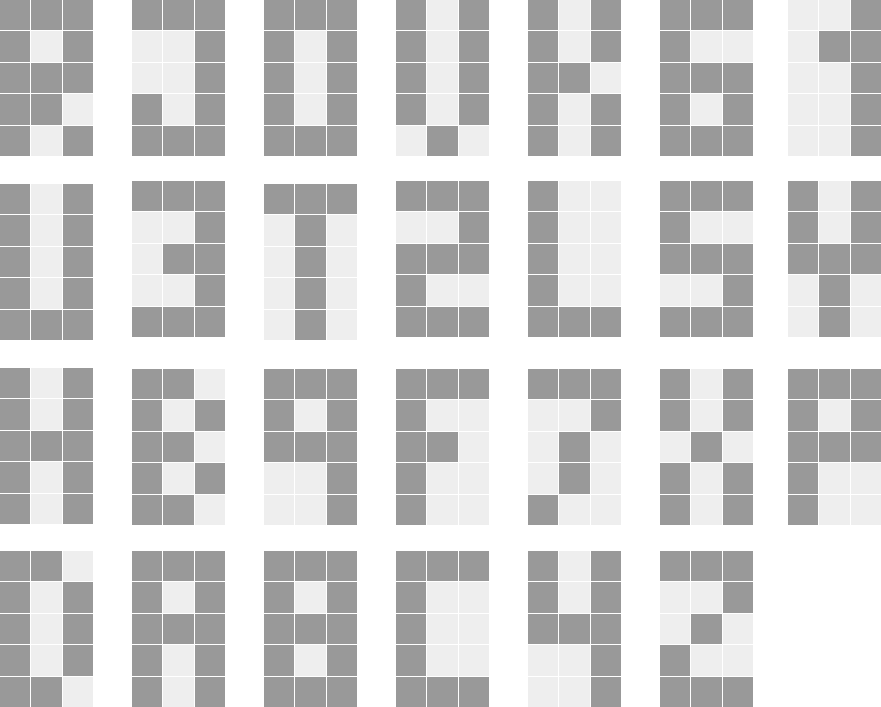
\includegraphics[width=\textwidth]{images/5.png}